\documentclass[11pt,a4paper]{article}
\usepackage[utf8]{inputenc}
\usepackage[vietnamese]{babel}
\usepackage{amsmath,amssymb}
\usepackage[version=4]{mhchem}
\usepackage{geometry}
\geometry{top=0.55cm,bottom=0.55cm,left=1.20cm,right=1.20cm,headheight=26pt,headsep=2pt,footskip=13pt}
\usepackage{graphicx}
\usepackage{xcolor}
\usepackage{tabularx}
\usepackage{array}
\usepackage{tikz}
\usepackage{multicol}
\usepackage{fancyhdr}
\usepackage{enumitem}

\definecolor{hfRed}{HTML}{D32F2F}
\definecolor{hfGreen}{HTML}{8BC390}
\definecolor{mainGreen}{HTML}{2E7D32}

\usepackage{ex_test}

\pagestyle{fancy}
\fancyhf{}
\renewcommand{\headrulewidth}{0.75pt}
\renewcommand{\headrule}{\hbox to\headwidth{\color{hfGreen}\leaders\hrule height \headrulewidth\hfill}}
\renewcommand{\footrulewidth}{0.75pt}
\renewcommand{\footrule}{\hbox to\headwidth{\color{hfGreen}\leaders\hrule height \footrulewidth\hfill}}

\fancyhead[L]{\small\itshape\color{hfRed}Tài liệu lưu hành nội bộ}
\fancyhead[R]{\small\color{hfRed}Thầy \textbf{TRẦN VĂN THẠNH} - 0777.470.803}

\fancyfoot[L]{\footnotesize\itshape\color{hfRed}CS1: 6/15 Nguyễn Hoàng, P. Kim Long, TP Huế \quad|\quad CS2: 24 Đặng Thái Thân, TP Huế}
\fancyfoot[R]{\small\textbf{\color{hfRed}Trang \thepage}}

\setlength{\parindent}{0pt}
\setlength{\parskip}{0.0pt}

\begin{document}

\begin{minipage}[t]{0.45\textwidth}
\textbf{SỞ GD\&ĐT THỪA THIÊN HUẾ}\\
\textbf{TRƯỜNG THPT HAI BÀ TRƯNG}\\
\textit{ĐỀ CHÍNH THỨC}\\
\textit{(Đề thi có 04 trang)}
\end{minipage}
\hfill
\begin{minipage}[t]{0.52\textwidth}
\raggedleft
\textbf{\color{hfRed}ĐỀ KIỂM TRA CHƯƠNG 8 -- NĂM HỌC 2026 - 2027}\\
\textbf{MÔN: HOÁ HỌC -- KHỐI 12}\\
\textit{Thời gian làm bài: 50 phút (không kể thời gian phát đề)}\\
\textbf{MÃ ĐỀ THI: 124}
\end{minipage}

\vspace{2pt}
\noindent
\textit{Họ, tên thí sinh:} \dotfill \textit{Lớp:} \dotfill \textit{SBD:} \dotfill

\vspace{1pt}
\noindent
\textit{\footnotesize (Cho biết nguyên tử khối: H = 1; C = 12; N = 14; O = 16; Na = 23; Mg = 24; Al = 27; S = 32; Cl = 35,5; K = 39; Ca = 40; Ti = 48; Cr = 52; Mn = 55; Fe = 56; Ni = 58,7; Cu = 64; Zn = 65; Ag = 108; Ba = 137; Pt = 195).}

\vspace{2pt}
\noindent
\textbf{PHẦN I (4,5 điểm -- 18 câu): Câu trắc nghiệm nhiều phương án lựa chọn.}\\
\textit{Thí sinh trả lời từ câu 1 đến câu 18. Mỗi câu hỏi thí sinh chỉ chọn một phương án.}

\Opensolutionfile{ans}[ans-de24-hs]

\begin{ex}
[KNTT - SBT] Nguyên tử Cr có cấu hình electron ở trạng thái cơ bản là $\text{[Ar]}3d^5 4s^1$. Trong phản ứng hoá học, khi nguyên tử Cr nhường đi 3 electron để tạo thành ion $\ce{Cr^3+}$, số electron còn lại trên phân lớp 3d là
\choice
{5.}
{4.}
{3.}
{2.}
\loigiai{}
\end{ex}

\begin{ex}
[KNTT - SBT] Dung dịch nào sau đây có màu vàng chanh?
\choice
{\ce{CuSO4}.}
{\ce{FeCl3}.}
{\ce{KMnO4}.}
{\ce{FeSO4}.}
\loigiai{}
\end{ex}

\begin{ex}
[KNTT - SBT] Dãy kim loại nào sau đây sắp xếp theo thứ tự tăng dần nhiệt độ nóng chảy?
\choice
{Na, Fe, Mg.}
{Na, Mg, Fe.}
{Fe, Mg, Na.}
{Mg, Fe, Na.}
\loigiai{}
\end{ex}

\begin{ex}
[CTST - SBT] Dung dịch muối chromium(III) sulfate có lẫn copper(II) sulfate, sử dụng dung dịch nào sau đây có thể loại bỏ nguyên tố copper ra khỏi muối chromium(III) sulfate?
\choice
{Dung dịch ammonia.}
{Dung dịch xút.}
{Dung dịch barium chloride.}
{Dung dịch soda.}
\loigiai{}
\end{ex}

\begin{ex}
Phức chất là gì?
\choice
{Phức chất là những hợp chất có cấu tạo rất phức tạp.}
{Phức chất là những chất gồm nhiều phân tử chất đơn giản kết hợp lại.}
{Phức chất là những chất được tạo thành từ hai hay nhiều phân tử muối.}
{Phức chất là những chất khi phân li trong dung dịch tạo thành các ion phức tồn tại độc lập và có tính chất xác định.}
\loigiai{}
\end{ex}

\begin{ex}
Cho phát biểu sau: “Phức chất đơn giản thường có một.(1). liên kết với các phối tử bao quanh. Liên kết giữa nguyên tử trung tâm và phối tử trong phức chất là liên kết.(2).”. Cụm từ cần điền vào (1) và (2) lần lượt là
\choice
{cation kim loại, ion.}
{nguyên tử kim loại, cho -- nhận.}
{nguyên tử trung tâm, cho -- nhận.}
{phối tử, ion.}
\loigiai{}
\end{ex}

\begin{ex}
Phức chất nào sau đây chứa ion phức có số phối trí là 4?
\choice
{$\ce{[Zn(NH3)4]^2+}$.}
{$\ce{[Ag(NH3)2]+}$.}
{$\ce{[Co(NH3)6]^3+}$.}
{$\ce{[Ni(CN)4]^2-}$.}
\loigiai{}
\end{ex}

\begin{ex}
Trong phức chất $\ce{[Cr(H2O)6]Cl3}$, ion phức có dạng hình học gì?
\choice
{Hình vuông.}
{Lập phương.}
{Hình bát diện.}
{Hình tứ diện.}
\loigiai{}
\end{ex}

\begin{ex}
Chọn phát biểu sai:
\choice
{Phức chất có thể mang điện tích hoặc không mang điện tích.}
{Phức chất mà nguyên tử trung tâm tạo 4 liên kết với các phối tử luôn có dạng hình học là tứ diện.}
{Giống như phân tử ammonia, phân tử methylamine cũng có thể đóng vai trò là phối tử do có cặp electron chưa liên kết.}
{Phức có 4 phối tử và nguyên tử trung tâm có AO $d^8$ sẽ có dạng hình học vuông phẳng.}
\loigiai{}
\end{ex}

\newpage

\begin{ex}
Trong phương trình hoá học dạng tổng quát của phức chất aqua: $\ce{M^{n+}(aq) + m H2O(l) -> [M(OH2)_m]^{n+}(aq)}$. Giá trị $n$ là:
\choice
{số electron hoá trị của cation kim loại M.}
{giá trị điện tích của cation kim loại M.}
{số electron độc thân của cation kim loại M.}
{hoá trị của cation kim loại M.}
\loigiai{}
\end{ex}

\begin{ex}
Phản ứng tạo phức chất thường có một số dấu hiệu dễ quan sát như
\choice
{sự hoà tan, sự ngưng tụ.}
{sự biến đổi màu sắc, sự thay đổi nhiệt độ nóng chảy.}
{sự biến đổi màu sắc, sự hoà tan, sự kết tủa.}
{sự hoà tan, sự thay đổi nhiệt độ sôi.}
\loigiai{}
\end{ex}

\begin{ex}
Cho dung dịch ammonia dư vào dung dịch chứa phức chất $\ce{[Ni(OH2)6]^2+}$ và anion $\ce{Cl-}$, có phản ứng: $\ce{[Ni(OH2)6]^2+(aq) + 6NH3(aq) -> [Ni(NH3)6]^2+(aq) + 6H2O(l)}$ (*). Phát biểu nào sau đây không đúng?
\choice
{Trong điều kiện của phản ứng (*), phức chất $\ce{[Ni(NH3)6]^2+}$ kém bền hơn phức chất $\ce{[Ni(OH2)6]^2+}$.}
{Phản ứng (*) là phản ứng thế phối tử.}
{Dung dịch sau phản ứng có $\text{pH} > 7$.}
{Trong phản ứng không có sự thay đổi số oxi hoá của các nguyên tố.}
\loigiai{}
\end{ex}

\begin{ex}
Nhỏ vài giọt dung dịch \ce{NH3} vào dung dịch \ce{CuSO4} loãng thấy xuất hiện kết tủa màu xanh nhạt, chứng tỏ phức chất $\ce{[Cu(OH)2(H2O)4]}$ đã được tạo thành. Tiếp tục nhỏ vào ống nghiệm dung dịch \ce{NH3} đến dư thấy kết tủa tan, đồng thời dung dịch chuyển sang màu xanh lam, chứng tỏ phức chất $\ce{[Cu(NH3)4(H2O)2]^2+}$ đã được tạo thành. Dấu hiệu của phản ứng tạo phức trên dựa vào:
\choice
{sự biến đổi màu sắc.}
{sự biến đổi màu sắc và sự hoà tan.}
{sự hoà tan.}
{sự kết tủa.}
\loigiai{}
\end{ex}

\begin{ex}
Phản ứng chuẩn độ $\ce{Fe^2+}$ trong dung dịch acid bằng dung dịch \ce{KMnO4} được biểu diễn bởi phương trình ion rút gọn sau: $\ce{MnO4-(aq) + 5Fe^2+(aq) + 8H+(aq) -> Mn^2+(aq) + 5Fe^3+(aq) + 4H2O(l)}$. Chất oxi hoá trong phản ứng trên là
\choice
{$\ce{Fe^2+(aq)}$.}
{$\ce{Mn^2+(aq)}$.}
{$\ce{MnO4-(aq)}$.}
{$\ce{H+(aq)}$.}
\loigiai{}
\end{ex}

\begin{ex}
Có thể loại bỏ sắt trong nước ngầm bằng cách đưa nước ngầm lên các bể lắng, lọc và sục không khí vào. Khi đó $\ce{Fe^2+}$ trong nước ngầm bị chuyển thành $\ce{Fe(OH)3}$ và lắng xuống. Chất oxi hoá $\ce{Fe^2+}$ thành $\ce{Fe(OH)3}$ là
\choice
{khí \ce{O2}.}
{khí \ce{N2}.}
{nước và khí \ce{O2}.}
{khí \ce{O2} và \ce{OH-}.}
\loigiai{}
\end{ex}

\begin{ex}
\begin{minipage}[t]{0.74\textwidth}
Phức chất $\ce{[Fe(OH2)6]^3+}$ có cấu tạo như hình bên. Số liên kết cho -- nhận mà nguyên tử trung tâm iron tạo được với các phối tử $\ce{OH2}$ là
\choice
{5.}
{4.}
{3.}
{6.}
\end{minipage}\hfill
\begin{minipage}[t]{0.24\textwidth}
\centering\vspace{0pt}
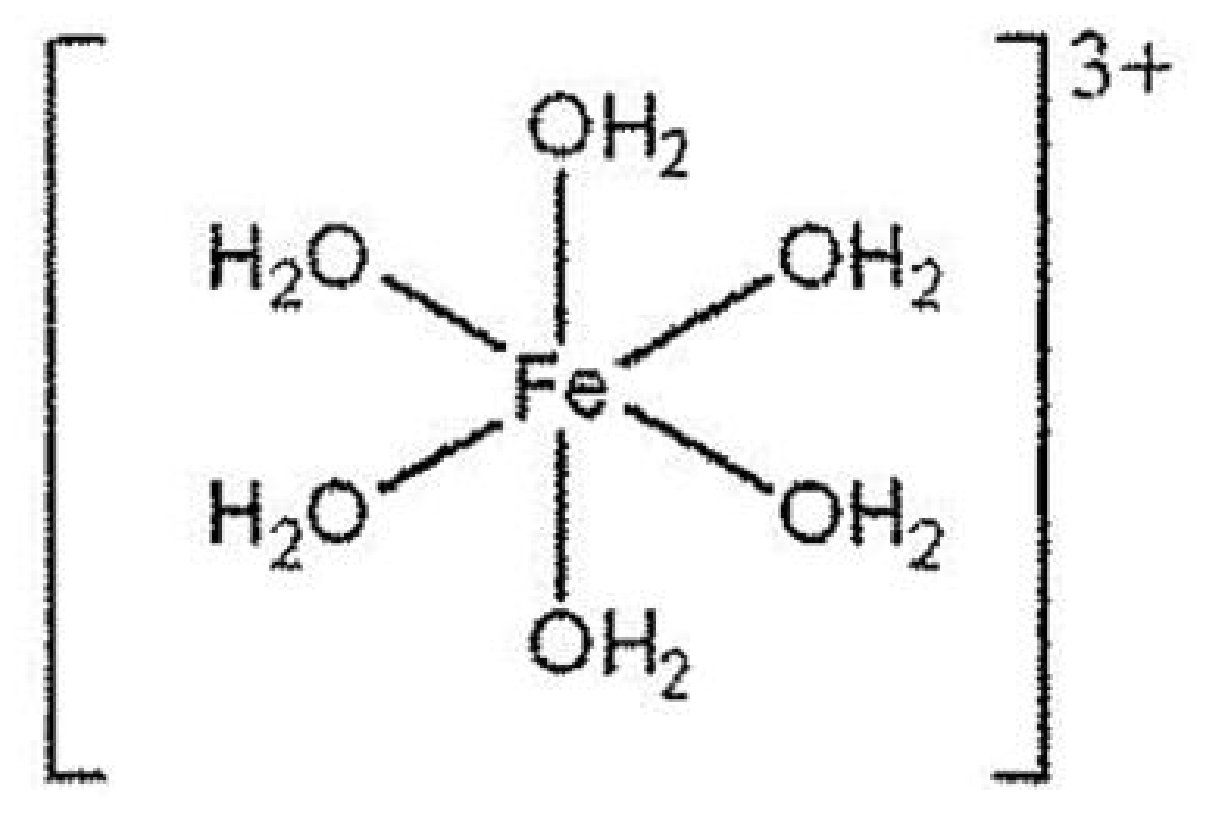
\includegraphics[width=\linewidth]{images_crop_de24/p1_cau16_fe_oh2_6.png}
\end{minipage}
\end{ex}

\begin{ex}
Trong các số oxi hoá của các kim loại chuyển tiếp dãy thứ nhất, trạng thái thường gặp nhất là +2. Điều này được giải thích là do đa số các kim loại chuyển tiếp dãy thứ nhất có độ âm điện không cao và
\choice
{dễ nhường đi 2 electron ở phân lớp 3d.}
{dễ nhường đi 1 electron ở phân lớp 3d và 1 electron ở phân lớp 4s.}
{có khả năng nhận thêm 2 electron vào phân lớp 3d.}
{có 2 electron lớp ngoài cùng.}
\loigiai{}
\end{ex}

\begin{ex}
Một học sinh tiến hành chuẩn độ dung dịch $\ce{Fe^2+}$ bằng dung dịch \ce{KMnO4} theo 2 cách:\\
-- \textit{Cách 1:} Nhỏ từ từ dung dịch \ce{KMnO4} vào dung dịch $\ce{Fe^2+}$ trong acid đến khi xuất hiện màu hồng nhạt bền khoảng 30 giây.\\
-- \textit{Cách 2:} Nhỏ từ từ dung dịch $\ce{Fe^2+}$ trong acid vào dung dịch \ce{KMnO4} đến khi màu hồng biến mất.\\
Cách tiến hành chuẩn độ nào là phù hợp?
\choice
{Cách 1.}
{Cách 2.}
{Cả hai cách.}
{Không có cách nào.}
\loigiai{}
\end{ex}

\newpage

\noindent
\textbf{PHẦN II (4,0 điểm -- 4 câu): Câu trắc nghiệm đúng sai.}\\
\textit{Thí sinh trả lời từ câu 1 đến câu 4. Trong mỗi ý a), b), c), d) ở mỗi câu, thí sinh chọn đúng hoặc sai.}

\setcounter{ex}{0}

\begin{ex}
\begin{minipage}[t]{0.70\textwidth}
Titanium (Ti) được sử dụng để chế tạo động cơ hoặc khung máy bay, còn titanium dioxide ($\ce{TiO2}$) được sử dụng trong sản xuất kem chống nắng. Quặng ilmenite ($\ce{FeTiO3}$) có giá trị quan trọng về mặt kinh tế để sản xuất kim loại titanium. $\ce{TiO2}$ sản xuất từ $\ce{FeTiO3}$ (phản ứng A), sau đó được chuyển hoá thành Ti theo quy trình Kroll (phản ứng B, C, D) như hình bên.\\
Xét tính đúng/sai của các phát biểu sau:
\choiceTF
{Phương trình hoá học của phản ứng A là: $\ce{FeTiO3 + C -> Fe + TiO2 + CO}$.}
{Phương trình hoá học của phản ứng B là: $\ce{TiO2 + 2Cl2 -> TiCl4 + O2}$.}
{Phương trình hoá học của phản ứng C là: $\ce{TiCl4 + 2Mg -> 2MgCl2 + Ti}$.}
{Phương trình tổng cộng của 4 phản ứng là: $\ce{FeTiO3 + 3C -> Fe + Ti + 3CO}$.}
\end{minipage}\hfill
\begin{minipage}[t]{0.28\textwidth}
\centering\vspace{0pt}
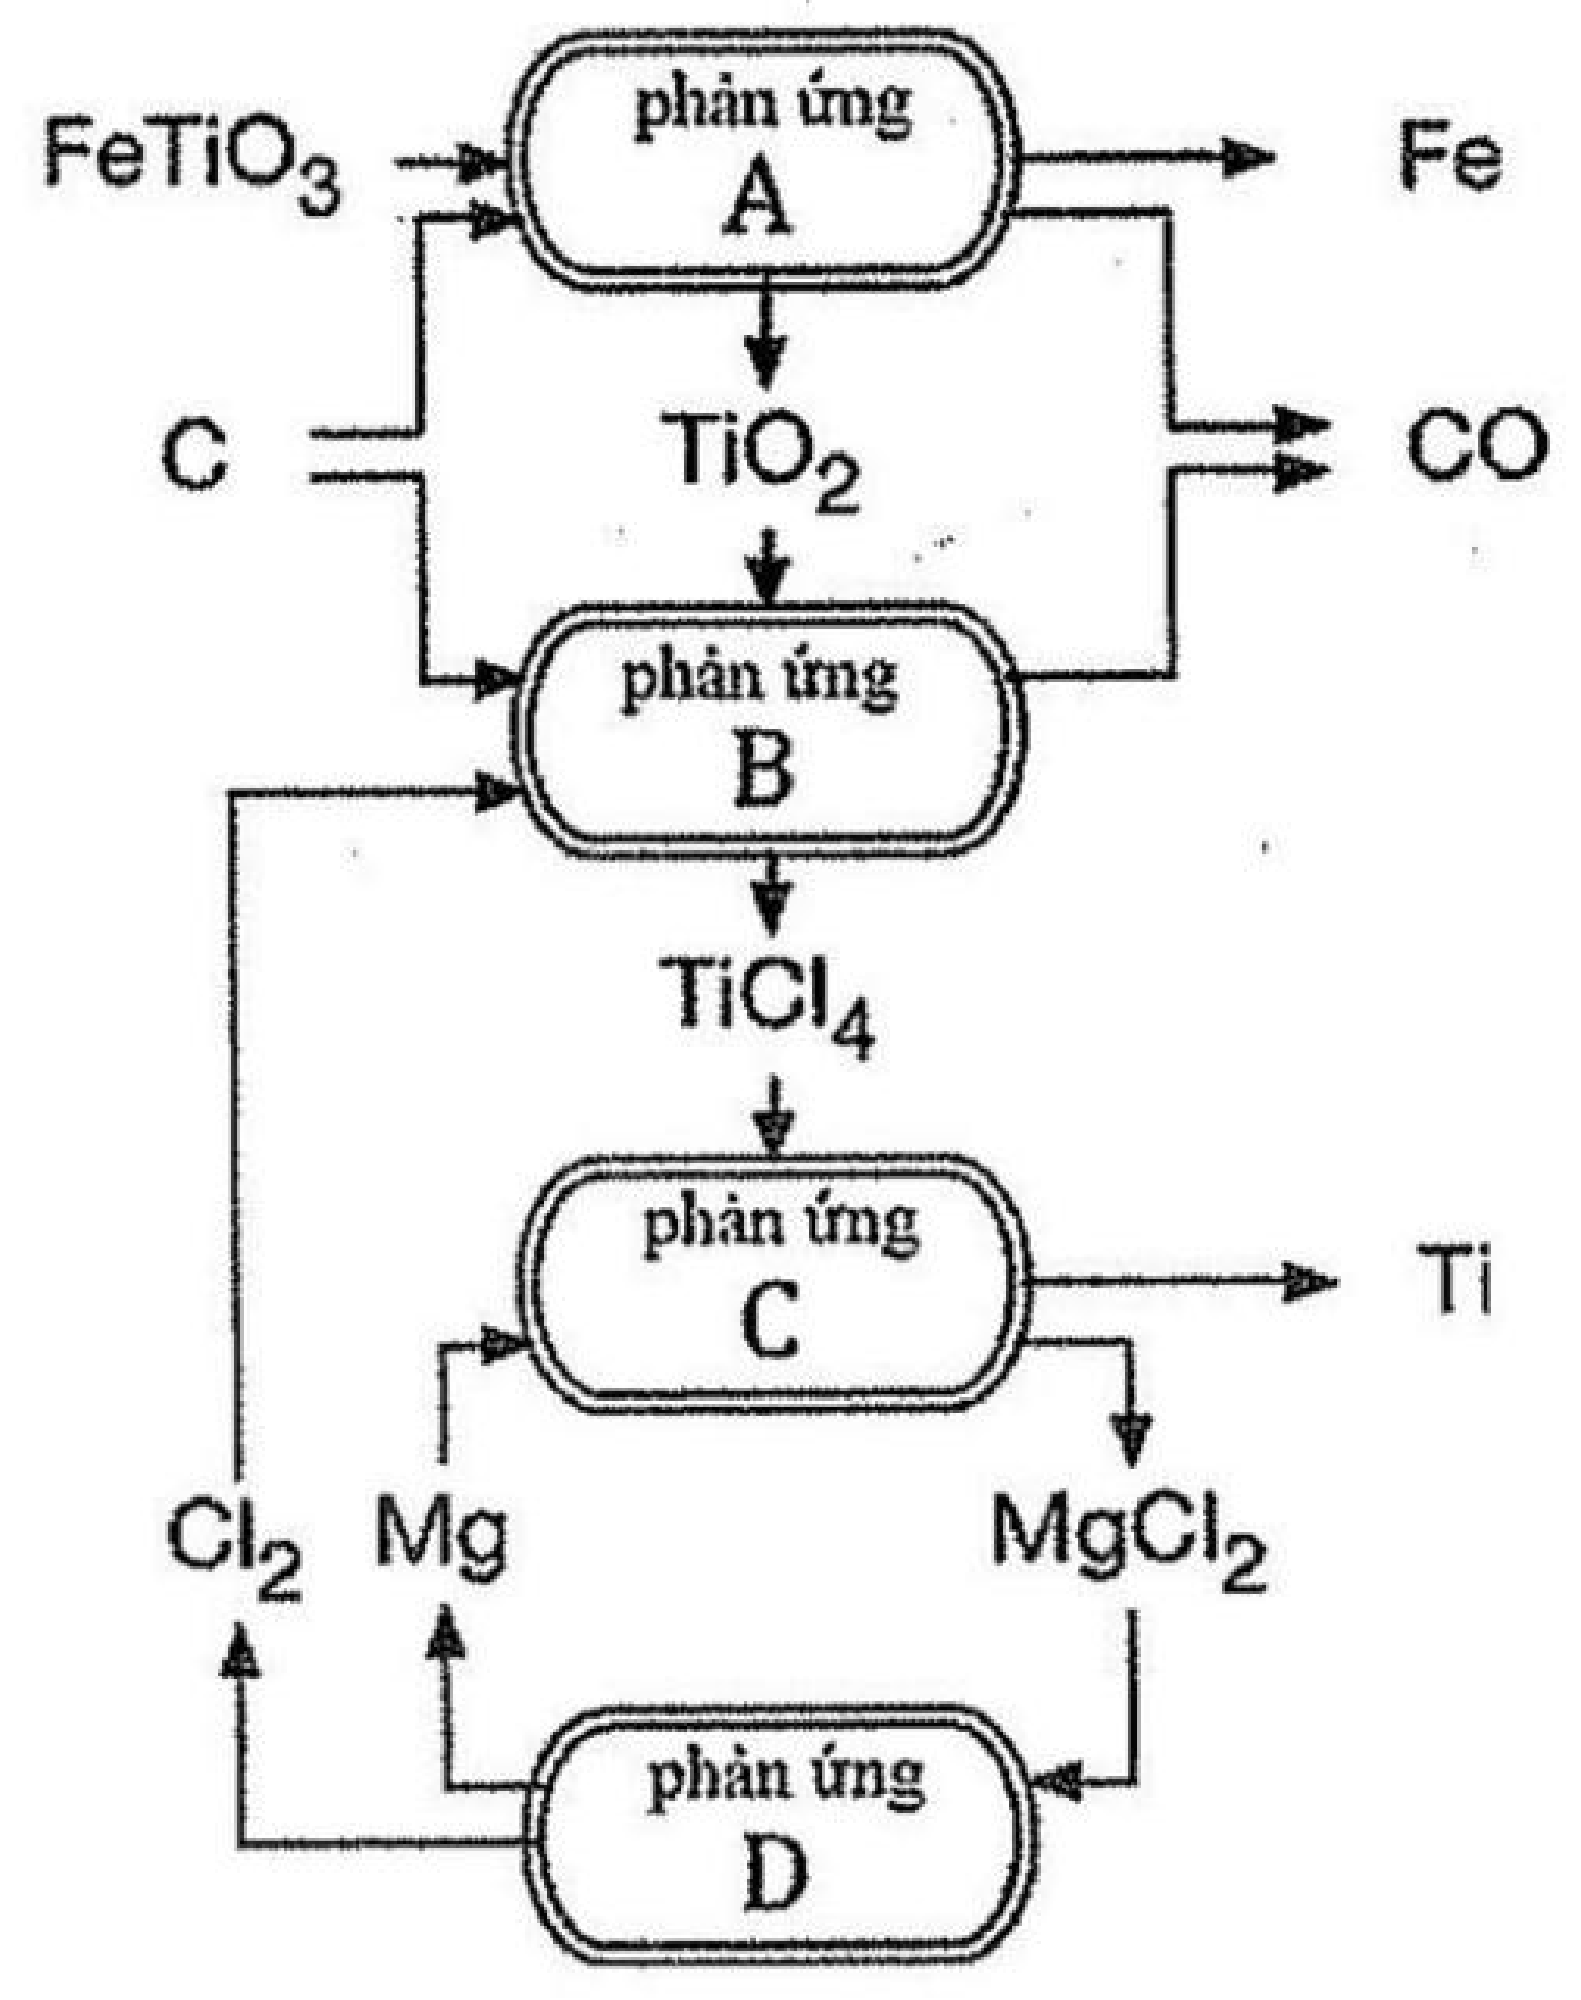
\includegraphics[width=\linewidth]{images_crop_de24/p2_cau1_quy_trinh_kroll.png}
\end{minipage}
\end{ex}

\begin{ex}
Phức chất \textit{cis}-$\ce{[Pt(NH3)2Cl2]}$ là một hợp chất vô cơ có khả năng ức chế các tế bào ung thư như ung thư tinh hoàn, buồng trứng, bàng quang và các khối u ở đầu và cổ. Mỗi phát biểu sau là đúng hay sai?
\choiceTF
{Ion trung tâm là Pt.}
{Phối tử là \ce{NH3}.}
{Ion trung tâm là $\ce{Pt^2+}$, phối tử là \ce{NH3} và \ce{Cl-}.}
{Phức có dạng hình học là vuông phẳng.}
\loigiai{}
\end{ex}

\begin{ex}
[KNTT - SBT] Trong dung dịch, ion $\ce{Fe^3+}$ tồn tại dưới dạng phức chất aqua có sáu phối tử nước. Xét tính đúng/sai của các phát biểu sau:
\choiceTF
{Phức chất aqua có công thức hoá học là $\ce{[Fe(H2O)6]^3+}$.}
{Phức chất aqua có dạng hình học vuông phẳng.}
{6 phối tử nước đã cho cặp electron chưa liên kết vào ion $\ce{Fe^3+}$.}
{Nguyên tử trung tâm trong phức chất aqua là $\ce{Fe^2+}$.}
\loigiai{}
\end{ex}

\begin{ex}
Cho hai phức chất A và B có công thức cấu tạo lần lượt sau:
\par\vspace{1pt}\centerline{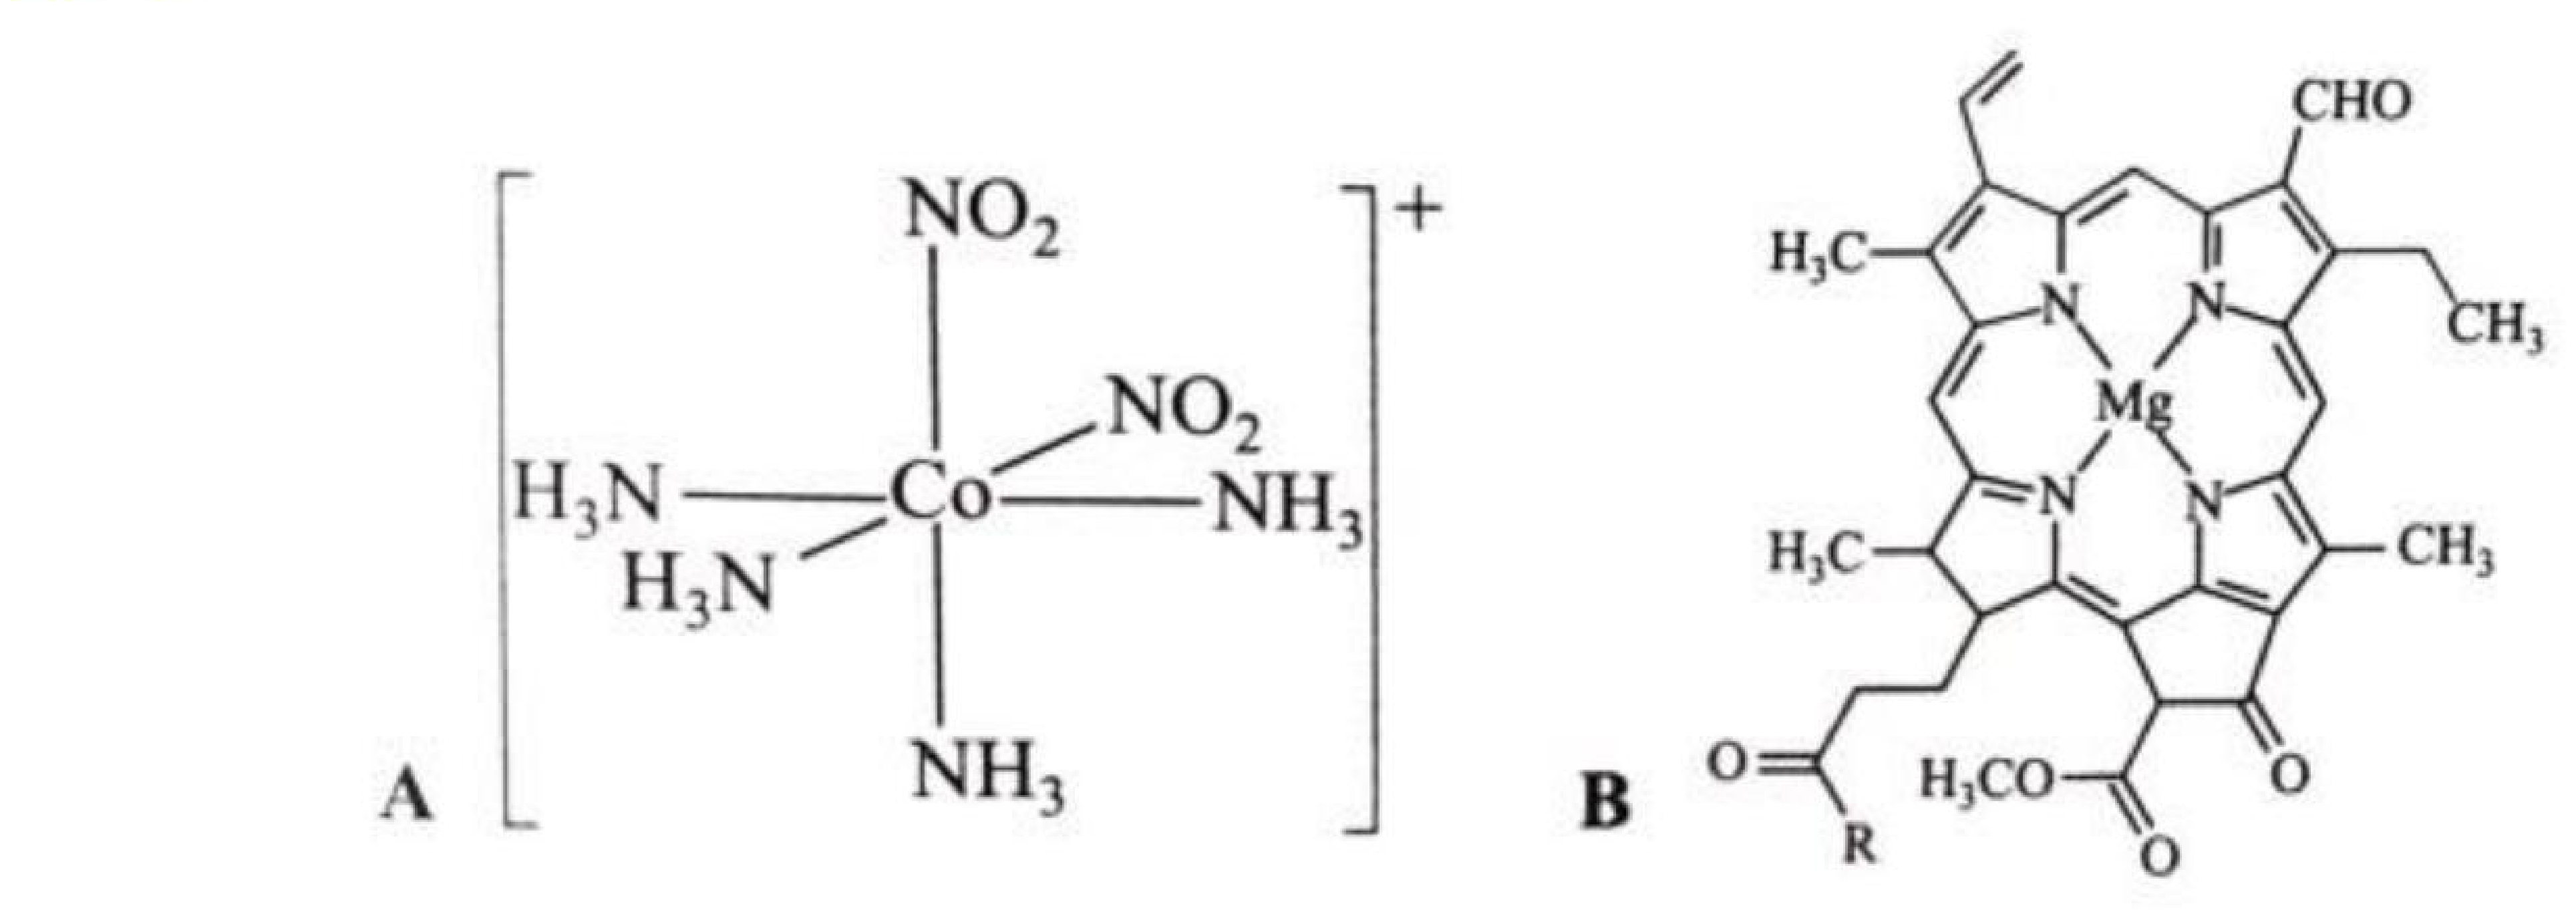
\includegraphics[height=2.3cm]{images_crop_de24/p2_cau4_phuc_A_B.png}}\vspace{1pt}
Mỗi phát biểu sau đây đúng hay sai?
\choiceTF
{Nguyên tử trung tâm của hai phức chất đều là nguyên tố kim loại chuyển tiếp.}
{Trong phức chất B có 4 phối tử.}
{Hai phức chất A và B có dạng hình học khác nhau.}
{Trong A và trong B đều có hai loại phối tử.}
\loigiai{}
\end{ex}

\newpage

\noindent
\textbf{PHẦN III (1,5 điểm -- 6 câu): Câu trắc nghiệm yêu cầu trả lời ngắn.}\\
\textit{Thí sinh trả lời từ câu 1 đến câu 6.}

\setcounter{ex}{0}

\begin{ex}
\begin{minipage}[t]{0.70\textwidth}
Phức chất $\ce{[Co(NH3)4Cl2]+}$ có cấu trúc như hình bên:\\
Có bao nhiêu liên kết sigma ($\sigma$) có trong phức chất đó?
\end{minipage}\hfill
\begin{minipage}[t]{0.28\textwidth}
\centering\vspace{0pt}
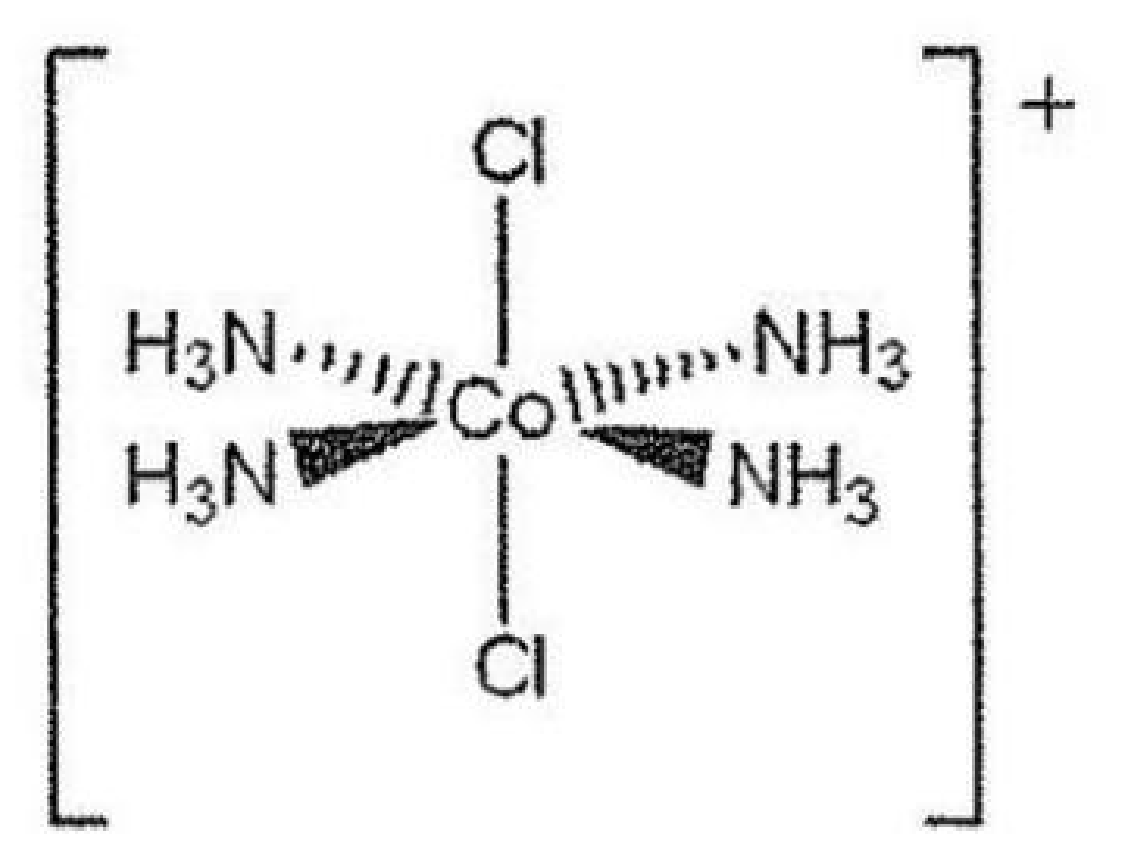
\includegraphics[height=1.8cm]{images_crop_de24/p3_cau1_co_nh3_4_cl2.png}
\end{minipage}
\end{ex}
\noindent\textit{Trả lời:} \dotfill
\vspace{0.2cm}

\begin{ex}
[KNTT - SBT] Phức chất $\ce{[MA_x B2]}$ có dạng hình học bát diện. Ở đó M là nguyên tử trung tâm, $x$ là số phối tử của A. Giá trị của $x$ là bao nhiêu?
\loigiai{}
\end{ex}
\noindent\textit{Trả lời:} \dotfill
\vspace{0.2cm}

\begin{ex}
[KNTT - SBT] Phức chất $\ce{[Co(NH3)Cl_x]^y-}$ có dạng hình học bát diện, nguyên tử trung tâm là $\ce{Co^3+}$. Tổng giá trị của $x$ và $y$ là bao nhiêu?
\loigiai{}
\end{ex}
\noindent\textit{Trả lời:} \dotfill
\vspace{0.2cm}

\begin{ex}
[KNTT - SBT] Cho dung dịch \ce{NH3} đặc vào dung dịch phức chất $\ce{[PtCl4]^2-}$ thu được phức chất có điện tích +1 là do một số phối tử \ce{Cl-} trong phức $\ce{[PtCl4]^2-}$ bị thay thế bởi phối tử \ce{NH3}. Số lượng phối tử \ce{Cl-} đã bị thay thế là bao nhiêu?
\loigiai{}
\end{ex}
\noindent\textit{Trả lời:} \dotfill
\vspace{0.2cm}

\begin{ex}
Sự gia tăng hàm lượng nitrate trong nước là một trong những nguyên nhân của hiện tượng phú dưỡng. Một trong những quy trình xác định hàm lượng nitrate trong nước được thực hiện như sau:\\
Thí nghiệm 1. Lấy 10,0 mL dung dịch muối Mohr [$\ce{(NH4)2SO4.FeSO4.6H2O}$], thêm $\ce{H2SO4}$ 1M vào và chuẩn độ bằng dung dịch \ce{KMnO4}.\\
Thí nghiệm 2. Lấy 10,0 mL dung dịch muối Mohr cho vào 100 mL nước chứa ion nitrate, sau đó thêm $\ce{NaOH(s)}$ vào để đạt khoảng 28\%, khi đó muối Mohr khử nitrate thành ammonia theo các phản ứng:\\
$\ce{NO3-(aq) + 2Fe(OH)2 + H2O -> NO2-(aq) + 2Fe(OH)3}$ (1)\\
$\ce{NO2-(aq) + 6Fe(OH)2 + 5H2O -> NH3 + 6Fe(OH)3 + OH-}$ (2)\\
Sau khi các phản ứng (1) và (2) hoàn toàn, lọc bỏ kết tủa, acid hoá dung dịch bằng dung dịch $\ce{H2SO4}$ 1M và chuẩn độ lượng $\ce{Fe^2+}$ dư bằng dung dịch \ce{KMnO4} (các chất và ion khác trong dung dịch không phản ứng với \ce{KMnO4}).\\
Hãy cho biết mỗi mmol \ce{KMnO4} chênh lệch giữa thí nghiệm 1 với thí nghiệm 2 sẽ tương ứng với bao nhiêu mg $\ce{NO3-}$ trong nước? \textit{(Làm tròn kết quả đến hàng phần mười)}.
\loigiai{}
\end{ex}
\noindent\textit{Trả lời:} \dotfill
\vspace{0.2cm}

\begin{ex}
Chromium (Cr) có tính cứng cao. Nickel (Ni) có đặc tính cơ học là cứng, dễ dát mỏng, dễ uốn, dễ kéo sợi và đặc tính hoá học là trơ với không khí nên khi thêm vào inox để việc gia công dễ dàng hơn. Inox 18/10 có thành phần hoá học gồm 18\% chromium, 10\% nickel và tối đa 0,08\% carbon (C). Xác định khối lượng iron (tính theo kg) tối đa trong 1,00 tấn inox 18/10.
\loigiai{}
\end{ex}
\noindent\textit{Trả lời:} \dotfill
\vspace{0.2cm}

\Closesolutionfile{ans}

\end{document}
